\documentclass[8pt]{beamer}

\newif\ifplacelogo % create a new conditional
\placelogotrue % set it to true

\usetheme{Warsaw}
\usecolortheme{rose}
\usepackage{multicol}
\usepackage{epstopdf}
\usepackage[italic]{hepnames}
\usepackage{tikz}
\usepackage{listings}
\usepackage{times}
\usepackage{amsmath}
\usepackage{verbatim}
\usepackage{hyperref}
\usepackage{bbding}
\lstset{breakatwhitespace,
language=C++,
columns=fullflexible,
keepspaces,
breaklines,
tabsize=3, 
showstringspaces=false,
extendedchars=true}

% TikZ includes!!!
\usepackage{tikz}
\usetikzlibrary{backgrounds}
\usetikzlibrary{calc}
\tikzstyle{every picture}+=[remember picture]
\input{/home/oviazlo/Desktop/beamerPresentations/myReports/latexHelpScripts/tikzGrid.tex}


\begin{document}

% custom colors
\definecolor{olive}{rgb}{0.3, 0.4, .1}
\definecolor{fore}{RGB}{249,242,215}
\definecolor{back}{RGB}{51,51,51}
\definecolor{title}{RGB}{255,0,90}
\definecolor{dgreen}{rgb}{0.,0.6,0.}
\definecolor{gold}{rgb}{1.,0.84,0.}
\definecolor{JungleGreen}{cmyk}{0.99,0,0.52,0}
\definecolor{BlueGreen}{cmyk}{0.85,0,0.33,0}
\definecolor{RawSienna}{cmyk}{0,0.72,1,0.45}
\definecolor{Magenta}{cmyk}{0,1,0,0}

\definecolor{PixelColor}{RGB}{207,232,139}
\definecolor{SCTColor}{RGB}{167,166,255}
\definecolor{TRTColor}{RGB}{250,224,140}
\definecolor{grayColor}{RGB}{153,153,153}

\newcommand{\yRefPosOne}{0.0}
\newcommand{\xRefPosOne}{0.0}
\newcommand{\yRefPosTwo}{0.0}
\newcommand{\xRefPosTwo}{0.0}
\newcommand{\yRefIncrementOne}{0.0}
\newcommand{\xRefIncrementOne}{0.0}
\newcommand{\yRefIncrementTwo}{0.0}
\newcommand{\xRefIncrementTwo}{0.0}

\graphicspath{ {/home/oviazlo/Desktop/beamerPresentations/FCCee/pictures/} }
\DeclareGraphicsExtensions{.eps, .pdf, .png}

\newcommand{\myBox}[2][pink] {
    \noindent\colorbox{#1}{
	\textbf{#2}
    }\par
}

% For nice block (provided by Oleh)
\tikzstyle{mybox} = [draw=red, fill=blue!1, very thick,
    rectangle, rounded corners, inner sep=5pt, inner ysep=9pt]
    
\tikzstyle{PixelBox} = [draw=PixelColor, fill=blue!1, very thick,
    rectangle, rounded corners, inner sep=5pt, inner ysep=9pt]
\tikzstyle{SCTBox} = [draw=SCTColor, fill=blue!1, very thick,
    rectangle, rounded corners, inner sep=5pt, inner ysep=9pt]
\tikzstyle{TRTBox} = [draw=TRTColor, fill=blue!1, very thick,
    rectangle, rounded corners, inner sep=5pt, inner ysep=9pt]

% poster advertisement
\newcommand{\myCenterBox}[2][pink] {
   {\centering
    \noindent\colorbox{#1}{
	\textbf{#2}
    }\par
  }
}

\newcommand{\mySmallCenterBox}[2][pink] {
   {\centering
    \noindent\colorbox{#1}{
	\textbf{{\small #2}}
    }\par
  }
}

\newcommand{\myVerySmallCenterBox}[2][pink] {
   {\centering
    \noindent\colorbox{#1}{
	\textbf{{\scriptsize #2}}
    }\par
  }
}

\newcommand{\backupbegin}{
   \newcounter{finalframe}
   \setcounter{finalframe}{\value{framenumber}}
}
\newcommand{\backupend}{
   \setcounter{framenumber}{\value{finalframe}}
}

\newcommand{\myNode}{\tikz[baseline,inner sep=1pt] \node[anchor=base]}

\definecolor{light-gray}{gray}{0.95}
% poster advertisement


\title[ Photon PID Efficiency with FCC-ee Detector \hspace{12.5em}\insertframenumber/
\inserttotalframenumber]{ Photon PID Efficiency with FCC-ee Detector }


	\author[Oleksandr Viazlo]{Oleksandr Viazlo \\ 
% 	{\small ???}
	}
	\institute{\small CERN\\} 
	
       
	\date{15 November 2017}

% 	\logo{ \ifplacelogo \includegraphics[height=1.8cm]{./ID_week2/lund_uni-logo_s.pdf} \hspace{0.4cm} \fi}

	
   	\frame{\titlepage}

   	

\placelogofalse

%*****************************************************************************
\begin{frame}{\large \large FCC-ee detector}
 
\renewcommand{\yRefPosOne}{0}
\renewcommand{\xRefPosOne}{5.3}
\renewcommand{\xRefIncrementOne}{5.5}
\begin{tikzpicture}[overlay]


\node [Box] at (\xRefPosOne-0.5,\yRefPosOne+3.1) (box){%
\begin{minipage}{1\textwidth}

 \begin{itemize}
  \item FCC-ee machine energy regimes: Z, WW, HZ, tt (91.2 - 365 GeV) \\[0.1cm]
  \item Detector design for FCC-ee is based on the CLIC detector \\[0.1cm]
 \end{itemize}
\end{minipage}
};

 \node[TRTBox] (tmp) at (\xRefPosOne,\yRefPosOne+0.3)
  { 
    \begin{minipage}{0.8\textwidth}

    \resizebox{\columnwidth}{!}{%
      \begin{tabular}{lccc}
	 & CLIC & & FCC-ee \\[0.18cm]
	VTX Barrel & 31-60 mm & $\Longrightarrow$ & 17-59 mm \\[0.18cm]
	Tracker radius & 1486 mm & $\Longrightarrow$ & 2100 mm \\[0.18cm]
	ECAL thickness & 40 layers, 22 X$_0$ & $\Longrightarrow$ & 40 layers, 22 X$_0$ \\[0.18cm]
	HCAL thickness & 60 layers, 7.5 $\lambda_I$ & $\Longrightarrow$ & 44 layers, 5.5 $\lambda_I$ \\[0.18cm]
	Solenoid field & 4 Tesla & $\Longrightarrow$ & 2 Tesla \\
	
      \end{tabular}%
    }
    \end{minipage}
  };
  
\node [Box] at (\xRefPosOne,\yRefPosOne+2.2) (box){%
\myCenterBox[TRTColor]{Overall dimensions of CLIC and FCC-ee detectors}
};
  
  
  \node [Box] at (\xRefPosOne-0.5,\yRefPosOne-3.3) (box){%
\begin{minipage}{1\textwidth}

 \begin{itemize}
  
  \item Standartd calorimeter calibration with 10 GeV photons, 10 GeV muons and\\ 50 GeV K0L, no software compensation
  \item Photon reconstruction training with Zuds 380 GeV sample
 \end{itemize}
\end{minipage}
};



  
\end{tikzpicture}
\end{frame}
%*****************************************************************************

%*****************************************************************************
\begin{frame}{\large \large Photon PID efficiency}
 
\renewcommand{\yRefPosOne}{0}
\renewcommand{\xRefPosOne}{5.3}
\renewcommand{\xRefIncrementOne}{5.5}
\begin{tikzpicture}[overlay]

\node [Box] at (\xRefPosOne-0.5,\yRefPosOne+1.5) (box){%
\begin{minipage}{1\textwidth}

 \begin{itemize}
%   \item Study of photon PID performance 
  \item Samples: photon gun with isotrop $cos(\theta)$ and $\phi$ distribution: \\1, 2, 5, 10, 20, 50, 100 GeV
  \item Efficiency definition: 
  \begin{itemize}
   \item correct reconstruction PFO type (pick most energetic PFO of correct type)
   \item energy matching: $|E_{MC}-E_{PFO}| < 200\% \times \sqrt{E_{MC}} + 0.5$GeV
  \end{itemize}

  
 \end{itemize}
\end{minipage}
};
 
   \node[inner sep=0pt] (tmp) at (\xRefPosOne-3,\yRefPosOne-2)
    {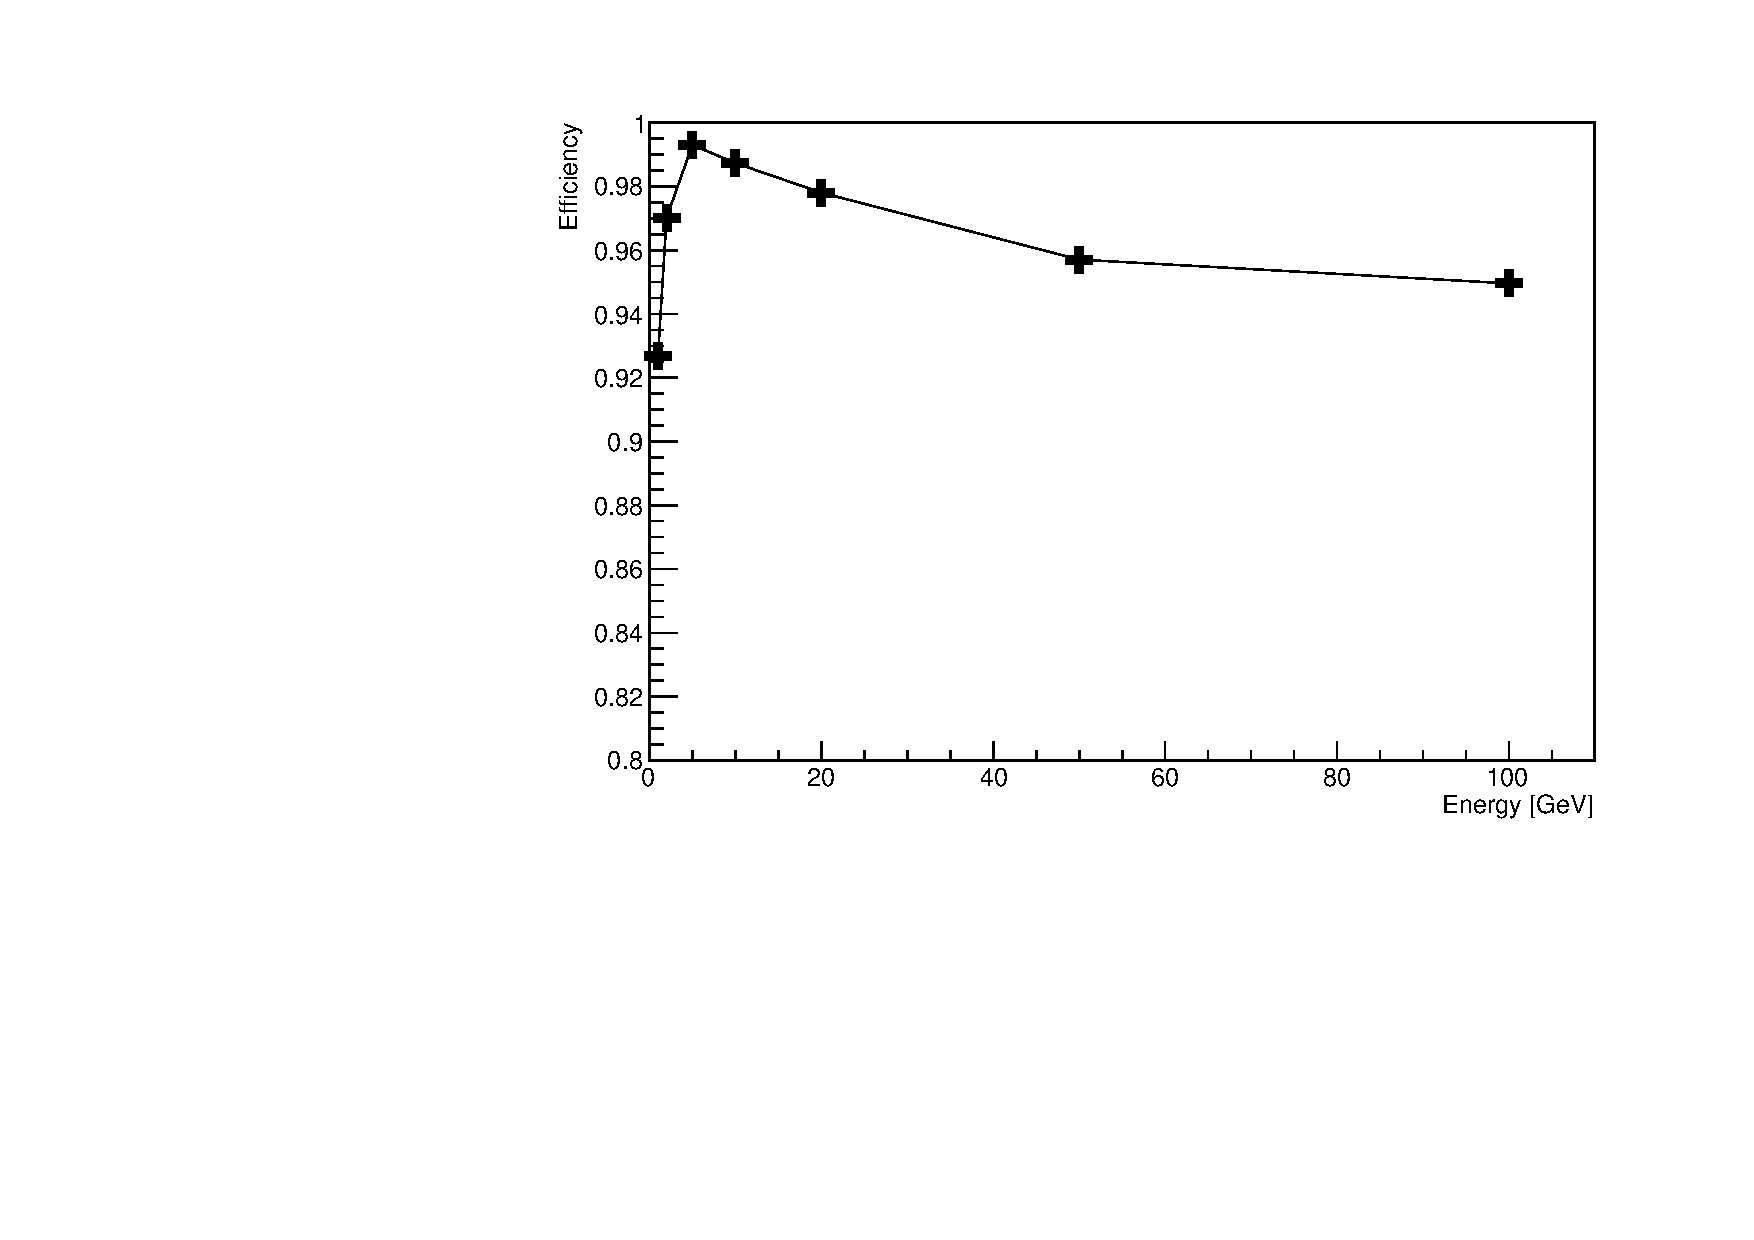
\includegraphics[width=6cm]{effPhoton_pandora.pdf}};
 
\node [Box] at (\xRefPosOne+5,\yRefPosOne-2) (box){%
\begin{minipage}{\textwidth}
{\small
\begin{tabular}{lccc}
  Energy & N_{total} & fail energy  & fail type \\
  $[$GeV$]$ & & matching & reconstruction \\
  \hline
  100 &	87249 &	3964 &	434 \\
  50 &	91116 &	3462 &	450 \\
  20 &	91121 &	1569 &	431 \\
  10 &	96993 &	652 &	576 \\
  5 &	99003 &	0 &	692 \\
  2 &	89121 &	0 &	2656 \\
  1 &	99027 &	0 &	7260 \\
\end{tabular}
}
\end{minipage}
};
 
 
\end{tikzpicture}
\end{frame}
%*****************************************************************************

%*****************************************************************************
\begin{frame}{\large \large Photon PID efficiency}
 
\renewcommand{\yRefPosOne}{0}
\renewcommand{\xRefPosOne}{5.3}
\renewcommand{\xRefIncrementOne}{5.5}
\begin{tikzpicture}[overlay]

   \node[inner sep=0pt] (tmp) at (\xRefPosOne-3,\yRefPosOne+0.5)
    {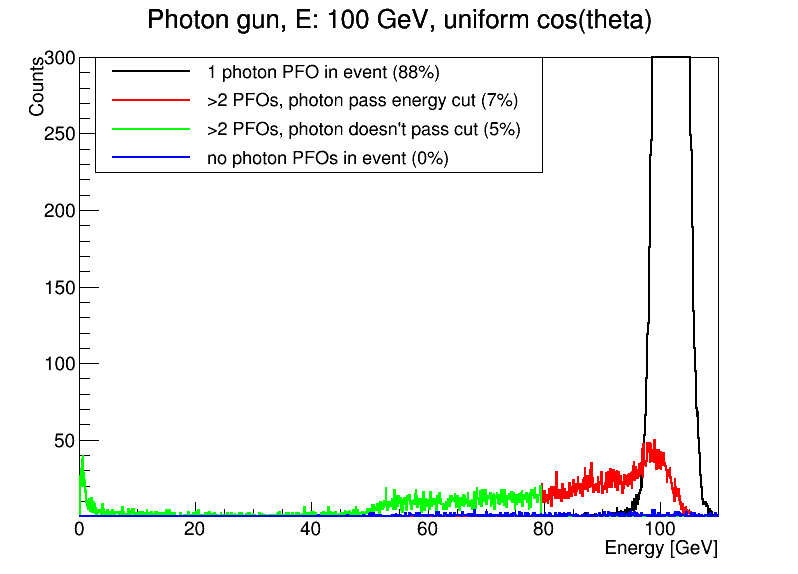
\includegraphics[width=6cm]{photon_100GeV.png}};
 
   \node[inner sep=0pt] (tmp) at (\xRefPosOne+3,\yRefPosOne+0.5)
    {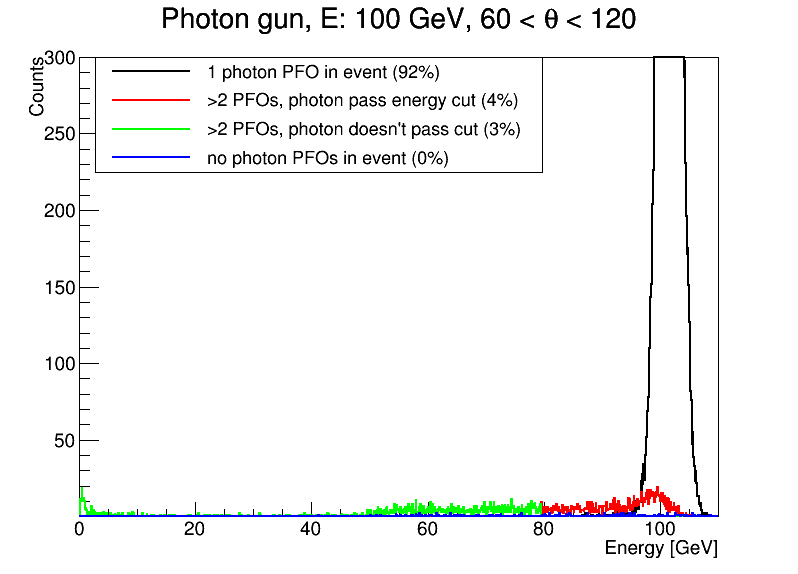
\includegraphics[width=6cm]{photon_100GeV_theta90.png}};
 
\node [Box] at (\xRefPosOne-0.5,\yRefPosOne-3) (box){%
\begin{minipage}{1\textwidth}

 \begin{itemize}
  \item Photon PFO reconstructed energy
  \item In $\simeq$10$\%$ of events two or more PFOs are found $\to$ 
        4-5$\%$ effect of photon efficiency loss
  \item Effect is smaller in only barrel region (60 $< \theta <$ 120) \\ [0.4cm]
  
  \item Is there a way to tune clustering algorithm?
  
 \end{itemize}
\end{minipage}
};
 
\end{tikzpicture}
\end{frame}
%*****************************************************************************

\end{document}

